\documentclass[crop, tikz]{standalone}
\usepackage{tikz, pgfplots}
\usepgfplotslibrary{groupplots}
\usepgfplotslibrary{fillbetween}
	
\begin{document}
	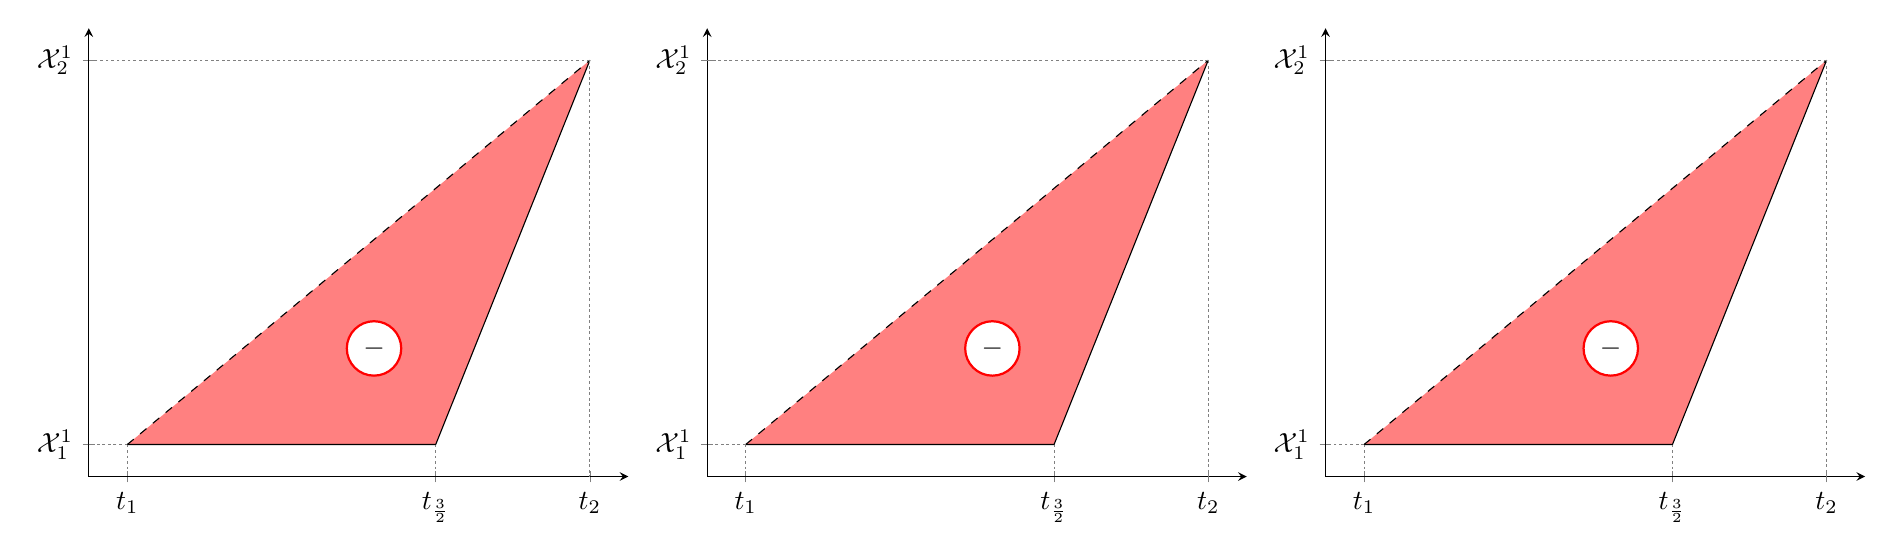
\begin{tikzpicture}[
		roundnode/.style={circle, draw=red, fill=white, thick},
	]
			
		\begin{groupplot}[
			group style = {
				group size = 3 by 1,
			}
		]
		
		% Add first group plot
		\nextgroupplot[
			xtick={0,2,3},
			xticklabels={
				$t_1$,
				$t_{\frac{3}{2}}$,
				$t_2$
				},
				ytick={0,3},
				yticklabels={
					$\mathcal{X}_1^1$,
					$\mathcal{X}_2^1$
				},
				enlargelimits=false,
				xmin=-0.25, xmax=3.25,
				ymin=-0.25, ymax=3.25,
				axis x line=bottom,
				axis y line=left,
			]
		
		% Add lower path	
\addplot[
	name path=A, 
	mark=none,
	]			
	coordinates {(0,0) (2,0) (3,3)};

		
% Add diagonal 
\addplot[
	name path=B,
	mark=none,
	dashed,
	]
	coordinates {(0,0) (3,3)};

% Add fill 	
\addplot[red!50] fill between[of=A and B];

% Add label
\node[roundnode] at (axis cs: 1.6, 0.75) {$-$};		

%\coordinate (p3) at (axis cs: 3,3);

% Add connectors		
\coordinate (p1) at (axis cs: 0,0);
\coordinate (pX11) at (axis cs: -1,0);
\coordinate (pt1) at (axis cs: 0,-1);
\draw[dash pattern=on 1pt off 1pt, gray] (p1) -- (pX11);
\draw[dash pattern=on 1pt off 1pt, gray] (p1) -- (pt1);

\coordinate (p2) at (axis cs: 2,0);
\coordinate (pt32) at (axis cs: 2,-1);
\draw[dash pattern=on 1pt off 1pt, gray] (p2) -- (pt32);

\coordinate (p3) at (axis cs: 3,3);
\coordinate (pX12) at (axis cs: -1,3);
\coordinate (pt2) at (axis cs: 3,-1);
\draw[dash pattern=on 1pt off 1pt, gray] (p3) -- (pX12);
\draw[dash pattern=on 1pt off 1pt, gray] (p3) -- (pt2);
		
		% Add second group plot
		\nextgroupplot[
		xtick={0,2,3},
		xticklabels={
			$t_1$,
			$t_{\frac{3}{2}}$,
			$t_2$
		},
		ytick={0,3},
		yticklabels={
			$\mathcal{X}_1^1$,
			$\mathcal{X}_2^1$
		},
		enlargelimits=false,
		xmin=-0.25, xmax=3.25,
		ymin=-0.25, ymax=3.25,
		axis x line=bottom,
		axis y line=left,
		]
		
		% Add lower path	
\addplot[
	name path=A, 
	mark=none,
	]			
	coordinates {(0,0) (2,0) (3,3)};

		
% Add diagonal 
\addplot[
	name path=B,
	mark=none,
	dashed,
	]
	coordinates {(0,0) (3,3)};

% Add fill 	
\addplot[red!50] fill between[of=A and B];

% Add label
\node[roundnode] at (axis cs: 1.6, 0.75) {$-$};		

%\coordinate (p3) at (axis cs: 3,3);

% Add connectors		
\coordinate (p1) at (axis cs: 0,0);
\coordinate (pX11) at (axis cs: -1,0);
\coordinate (pt1) at (axis cs: 0,-1);
\draw[dash pattern=on 1pt off 1pt, gray] (p1) -- (pX11);
\draw[dash pattern=on 1pt off 1pt, gray] (p1) -- (pt1);

\coordinate (p2) at (axis cs: 2,0);
\coordinate (pt32) at (axis cs: 2,-1);
\draw[dash pattern=on 1pt off 1pt, gray] (p2) -- (pt32);

\coordinate (p3) at (axis cs: 3,3);
\coordinate (pX12) at (axis cs: -1,3);
\coordinate (pt2) at (axis cs: 3,-1);
\draw[dash pattern=on 1pt off 1pt, gray] (p3) -- (pX12);
\draw[dash pattern=on 1pt off 1pt, gray] (p3) -- (pt2);
		
		% Add third group plot
		\nextgroupplot[
		xtick={0,2,3},
		xticklabels={
			$t_1$,
			$t_{\frac{3}{2}}$,
			$t_2$
		},
		ytick={0,3},
		yticklabels={
			$\mathcal{X}_1^1$,
			$\mathcal{X}_2^1$
		},
		enlargelimits=false,
		xmin=-0.25, xmax=3.25,
		ymin=-0.25, ymax=3.25,
		axis x line=bottom,
		axis y line=left,
		]
		
		% Add lower path	
\addplot[
	name path=A, 
	mark=none,
	]			
	coordinates {(0,0) (2,0) (3,3)};

		
% Add diagonal 
\addplot[
	name path=B,
	mark=none,
	dashed,
	]
	coordinates {(0,0) (3,3)};

% Add fill 	
\addplot[red!50] fill between[of=A and B];

% Add label
\node[roundnode] at (axis cs: 1.6, 0.75) {$-$};		

%\coordinate (p3) at (axis cs: 3,3);

% Add connectors		
\coordinate (p1) at (axis cs: 0,0);
\coordinate (pX11) at (axis cs: -1,0);
\coordinate (pt1) at (axis cs: 0,-1);
\draw[dash pattern=on 1pt off 1pt, gray] (p1) -- (pX11);
\draw[dash pattern=on 1pt off 1pt, gray] (p1) -- (pt1);

\coordinate (p2) at (axis cs: 2,0);
\coordinate (pt32) at (axis cs: 2,-1);
\draw[dash pattern=on 1pt off 1pt, gray] (p2) -- (pt32);

\coordinate (p3) at (axis cs: 3,3);
\coordinate (pX12) at (axis cs: -1,3);
\coordinate (pt2) at (axis cs: 3,-1);
\draw[dash pattern=on 1pt off 1pt, gray] (p3) -- (pX12);
\draw[dash pattern=on 1pt off 1pt, gray] (p3) -- (pt2);
		
		\end{groupplot}
	
	\end{tikzpicture}
\end{document}
	